\chapter{Аналитический раздел}
В данном разделе будет проанализирована поставленная задача, определён необходимый функционал програмного обеспечения, описаны роли пользователей программы и будет произведён анализ существующих моделей базы данных.

\section{Постановка задачи}
Необходимо разработать программу для отображения, манипуляции и эффективного хранения информации интернет-магазина парфюмерии. Покупатель должен иметь возможность просмотра каталога товаров, оформления зазаза выбранной продукции, написания отзывов к товарам и постановки оценок товарам и отзывам других покупетелей. Необходимо предусмотреть наличие ролей менеджера и администратора, осуществляющих модерацию и управление продукцией (добавление, изменение, удаление товаров), заказами(просмотр товаров, при необходимости корректировка заказа), модерации некорректных отзывов и регулярующих деятельность покупателей, в том числе доступ к профилям покупателей, при необходимости внесение корректировок или удаление профиля.
\section{Формализация данных}

\captionsetup{singlelinecheck = false, justification=raggedright}
\begin{table}[h!]
	\begin{center}
		\caption{Данные и сведения о них}
		\begin{tabular}{ |p{5cm}|p{11cm}| }
			\hline
			\textbf{Данные} & \textbf{Сведения}\\ \hline
			Пользователь &  ФИО, никнейм, дата рождения, адрес, e-mail, пароль, права доступа, пол, аватар\\ \hline
			Товар &  Заголовок, описание, фото, категории,\ количество, стоимость, дата публикации, объем флакона, рейтинг\\ \hline
			Заказ &  Товары, дата оформления, дата исполнения,\ стоимость, статус, комментарий\\ \hline
			Отзыв &  Содержание, дата, пользователь, рейтинг, дата\ публикации\\ \hline
			Оценка &  Дата, значение, пользователь\\ \hline
		\end{tabular}
		\label{data-table}
	\end{center}
\end{table}		

\newpage

\section{Типы пользователей}

\captionsetup{singlelinecheck = false, justification=raggedright}
\begin{table}[h!]
	\begin{center}
		\caption{Типы пользователей и их функционал}
		\begin{tabular}{ |p{5cm}|p{11cm}| }
			\hline
			\textbf{Тип пользователя} & \textbf{Функционал}\\ \hline
			Покупатель & Просмотр каталога продукции и информации о товарах, написание отзывов и постановка оценок товарам и комментариям\\ \hline
			Менеджер & Просмотр каталога продукции и информации о товарах\newline Просмотр информации покупателей, просмотр информации о заказах, подтверждение и отклонение заказов, обновление продукции и информации о ней, при необходимости модерация комментариев пользователей\\ \hline
			Администратор & Просмотр каталога продукции и информации о товарах\newline Просмотр информации покупателей, просмотр информации о заказах, подтверждение и отклонение заказов, обновление продукции и информации о ней, при необходимости модерация комментариев пользователей\newline Добавление и удаление менеджеров и возможность изменение информации пользователей, либо их удаление\\ \hline
		\end{tabular}
		\label{user-table}
	\end{center}
\end{table}		


На рисунке \ref{use_case} представлена Use-Case-диаграмма.

\section{ER-диаграмма сущностей}

На рисунке \ref{er_diagram} представлена ER-диаграмма сущностей проекта.

\captionsetup{singlelinecheck = false, justification=centering}
\begin{figure}[h!]
	\begin{center}
		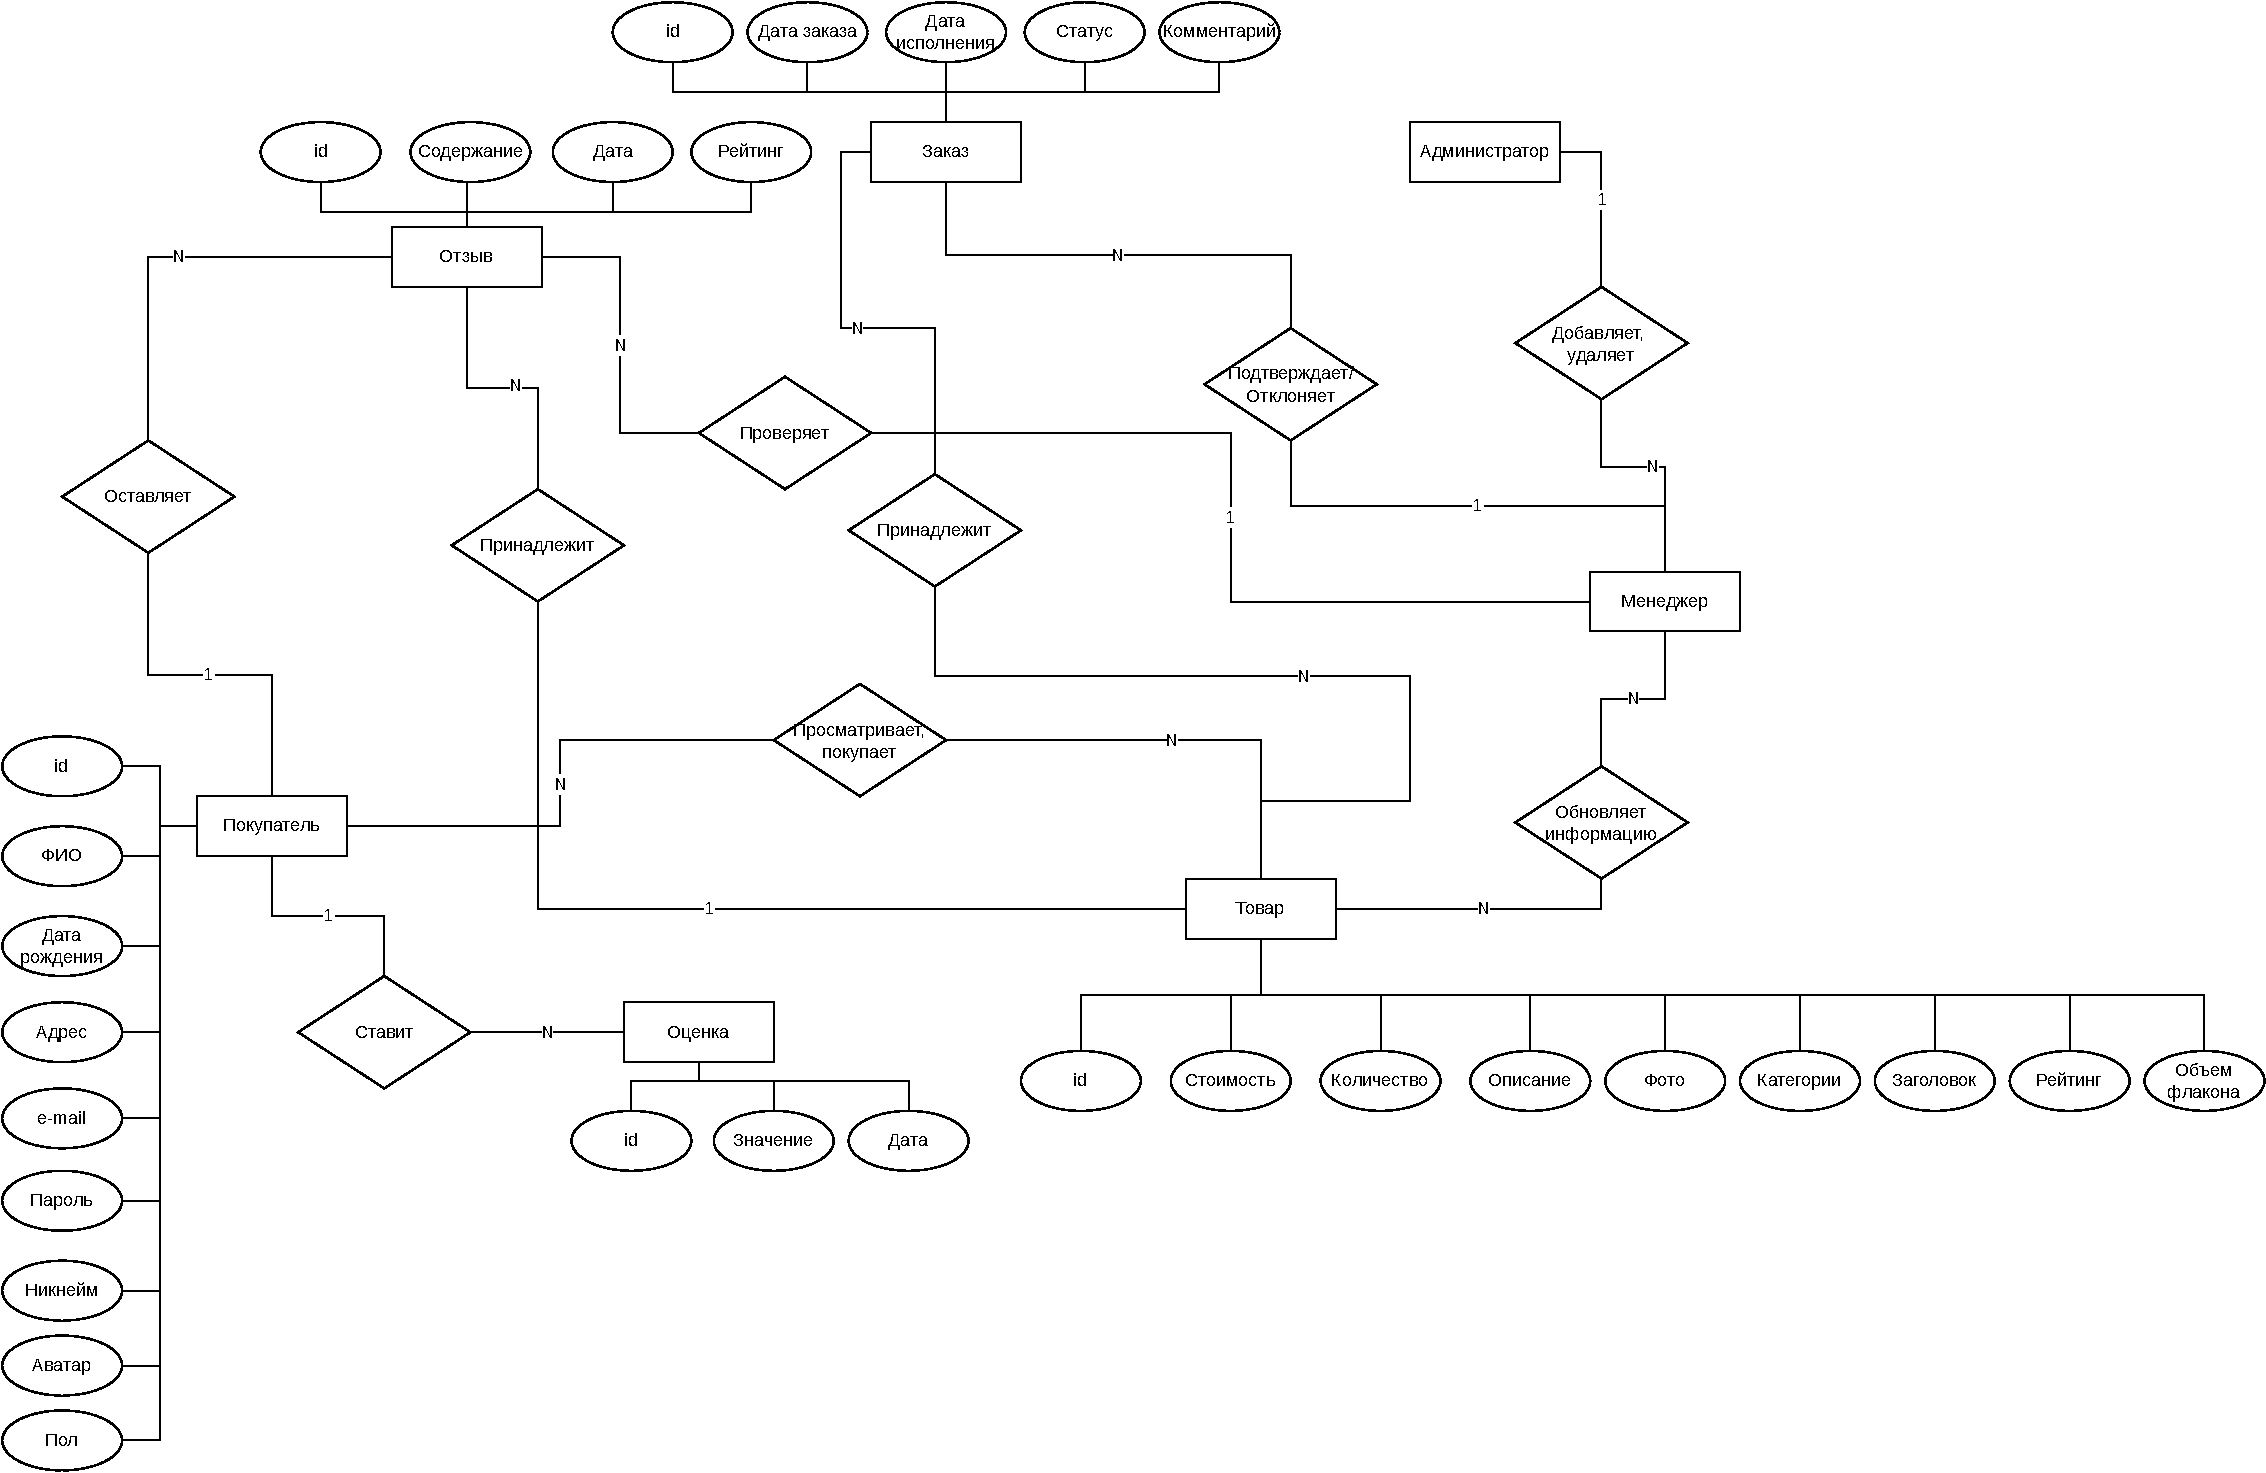
\includegraphics[scale=0.45, angle=90]{assets/er.pdf}
	\end{center}
	\caption{ER-диаграмма сущностей}
	\label{er_diagram}
\end{figure}

\captionsetup{singlelinecheck = false, justification=centering}
\begin{figure}[h!]
	\begin{center}
		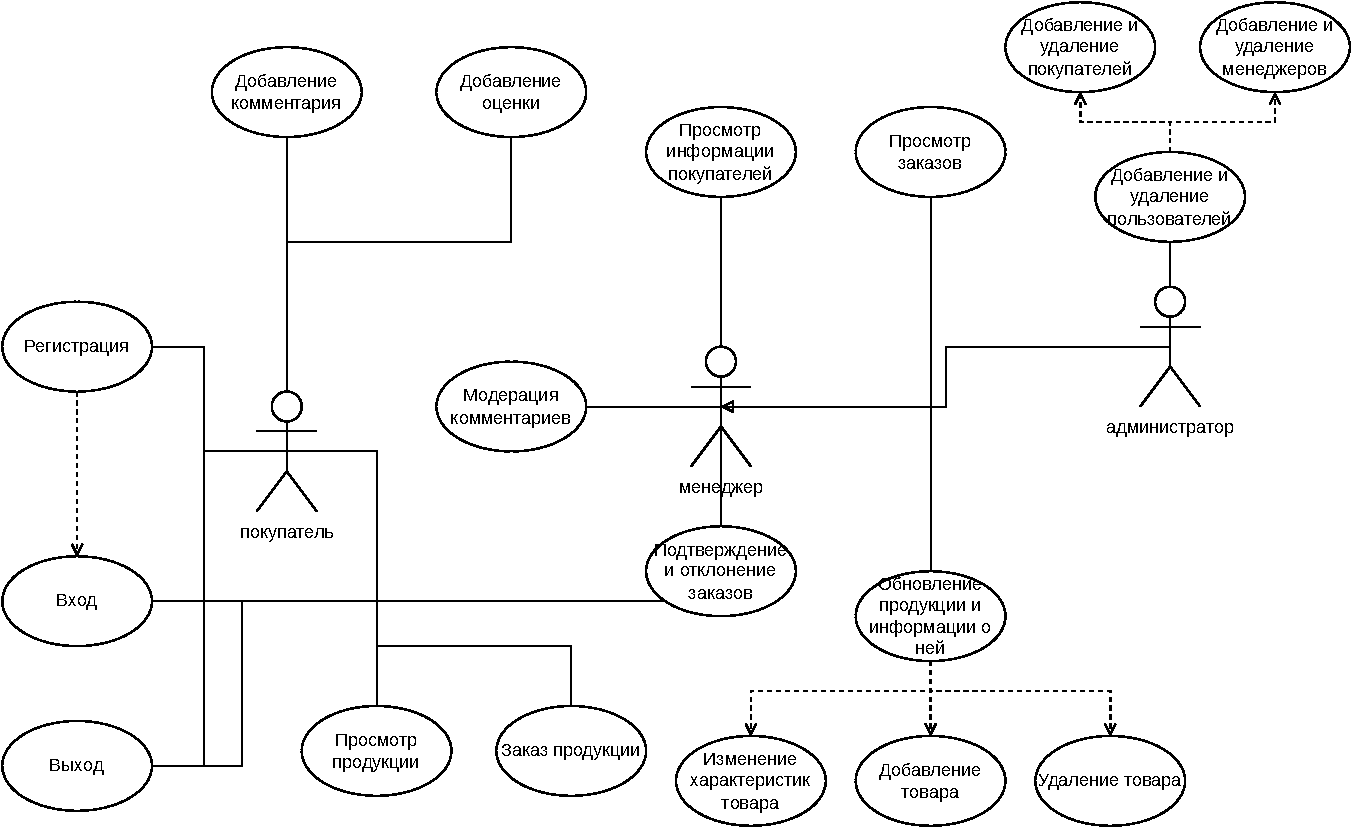
\includegraphics[scale=0.6]{assets/use_case.pdf}
	\end{center}
	\caption{Use-Case диаграмма}
	\label{use_case}
\end{figure}

\section{Описание существующих СУБД}
\textbf{Система управления базами данных} --- это комплекс языковых и программных средств, предназначенный для создания, ведения и совместного использования БД многими пользователями [1]. 

\subsection{Основные функции СУБД}
Основынми функциями СУБД являются:
\begin{itemize}
	\item cоздание, изменение и удаление структуры базы данных (таблиц, индексов, представлений и других объектов);
	\item организация и оптимизация хранения данных;
	\item реализация механизмов контроля целостности и согласованности данных (транзакции, ограничения, триггеры);
	\item обеспечение многопользовательского доступа к базе данных;
	\item мониторинг и управление производительностью базы данных;
	\item журнализация изменений, резервное копирование и восстановление базы данных после сбоев;
	\item поддержка языков БД.
\end{itemize}

\subsection{Классификация СУБД по модели данных}
\textbf{Модель данных} --- это абстрактное, самодостаточное, логическое определение объектов, операторов и прочих элементов, в совокупности составляющих абстрактную машину доступа к данным, с которой взаимодействует пользователь. Эти объекты позволяют моделировать структуру данных, а операторы --- поведение данных [2]. 

Основные типы моделей организации данных:
\begin{itemize}
	\item иерархическая
	
Модель данных, в основе которой лежит иерархическая структура типа дерева. Дерево --- это орграф, в каждую вершину которого кроме первой (корневой), входит только одна дуга, а из любой вершины (кроме конечных) может исходить произвольное число дуг. В иерархической структуре подчиненный элемент данных всегда связан только с одним исходным [3]. Но при том, что у каждого дочернего элемента может быть только один родительский, у родительского может быть несколько дочерних. 

Преимущества иерархической модели данных:
\begin{itemize}
	\item простая организация данных отражает их естественную иерархическую структуру;
	\item высокая производительность выполнения запросов, связанных с навигацией по иерархии;
\end{itemize}

Недостатки:
\begin{itemize}
	\item ограничение на количество связей между узлами. Множественные связи между двумя узлами не предусмотрены;
	\item сложность обновления данных, особенно в случае изменения структуры иерархии;
	\item отсутствие гибкости, так как система сильно зависит от текущей модели данных;
\end{itemize}

	\item сетевая
	
Основана на представлении информации в виде орграфа, в котором в каждую вершину может входить произвольное число дуг. Вершинам графа сопоставлены типы записей, дугам --- связи между ними [3]. В отличие от иерархической модели, где каждая запись может иметь только одного родителя, в сетевой модели запись может иметь несколько родительских записей и несколько дочерних записей.

Преимущества сетевой модели данных:
\begin{itemize}
	\item более гибкая структура данных по сравнению с иерархической моделью. Записи могут иметь несколько родителей, что позволяет представить более сложные связи между данными;
	\item высокая производительность при доступе к связанным данным, поскольку нет необходимости проходить через все уровни иерархии;
\end{itemize}

Недостатки:
\begin{itemize}
	\item сложность при проектировании и поддержке структуры данных, особенно при изменениях;
	\item зависимость от физической структуры данных и последовательности прочтения записей;
	\item ограниченная поддержка сложных запросов и агрегатных операций;
\end{itemize}

	\item графовая
	
Графовая модель данных основана на математической теории графов. В этой модели данные представляются в виде набора вершин (узлов) и связей (ребер), которые соединяют эти вершины. Каждая вершина может иметь атрибуты, которые хранят информацию о ней. Связи также имеют атрибуты и определяют отношения между вершинами. Главная особенность графовой модели данных состоит в том, что она позволяет представлять сложные связи и отношения между данными

Преимущества графовой модели данных:
\begin{itemize}
	\item гибкая структура данных, способствующая моделированию сложных отношений;
	\item эффективность при выполнении запросов, особенно связанных с обходом и анализом графовых структур;
	\item наглядность и понятность представления данных;
\end{itemize}

Недостатки:
\begin{itemize}
	\item нет единого языка запросов для графовых баз данных;
	\item затраты на хранение и обработку связей между вершинами, особенно в случае больших графовых структур;
\end{itemize}

	\item реляционная
	
В реляционной модели для отображения информации о предметной
области используется таблица, называемая отношением. Строка такой таблицы называется кортежем, столбец --- атрибутом. Каждый атрибут может принимать некоторое подмножество значений из определенной области --- домена.

Табличная организация БД позволяет реализовать ее важнейшее преимущество перед другими моделями данных, а именно возможность использования точных математических методов манипулирования данными,
и, прежде всего, аппарата реляционной алгебры и исчисления отношений.

К другим достоинствам реляционной модели можно отнести наглядность,
простоту изменения данных и организации разграничения доступа к ним [3]. 
\end{itemize}

\section*{Вывод}
\addcontentsline{toc}{section}{Вывод}

Поскольку реляционная модель базы данных является наиболее широко используемой и удобной, имеет возможность изменения базы данных без глобальных изменений программного обеспечения, а также обеспечивает поддержку ограничений, таких как ограничения целостности, что позволяет гарантировать, что данные, хранящиеся в базе данных, всегда являются корректными, то для реализации данного проекта была выброана именно она.

В данном разделе была произведена формализация поставленной задачи, описан необходимый функционал с распределением по ролям, проанализорованы модели базы данных и выбрана реляционная модель.